\documentclass[11pt,open=any]{scrreprt}

% Evan Chen's package provides the mathematical environments, theorem styling,
% typography, headers, colours, hyperlinks, and supporting utilities used here.
\usepackage[sexy]{evan}

% Additional packages needed by this report's tables and code listings.
\usepackage{booktabs}
\usepackage{longtable}
\usepackage{float}

\title{\textbf{\huge Segment Tree}\\[4pt]\large Fast Range Queries and Dynamic Updates}
\author{\textsc{Shayan Un Noor} (2305024) \\ \textsc{Md.\ Shadman Shahriyar Shuvo} (2305025) \\ \textsc{Md.\ Wasif Haque} (2305029)}
\date{}

\begin{document}
\maketitle
\thispagestyle{empty}
\vfill
\begin{center}
\textit{A technical report on hierarchical range-query data structures}
\end{center}
\clearpage
\pagenumbering{roman}
\tableofcontents
\listoffigures
\listoftables
\clearpage
\pagenumbering{arabic}

\begin{abstract}
\noindent Segment Trees are hierarchical data structures designed to efficiently process range queries and dynamic updates over an array. A na\"ive approach may require linear time for every range query or update, which becomes inefficient when the number of operations is large. A Segment Tree addresses this problem by recursively partitioning an array into smaller intervals and storing a summary of each interval at a tree node. This organization allows both point updates and range queries to be performed in $O(\log n)$ time after $O(n)$ preprocessing. This report presents the structure and construction of a Segment Tree, explains its update and query procedures using worked examples, derives their time complexities, and discusses its generalization to operations such as minimum, maximum, and greatest common divisor. The report also compares Segment Trees with Fenwick Trees and other conventional approaches.
\end{abstract}

% ============================================================
\chapter{Preliminaries and Terminology}

\subsection{Arrays, Intervals, and Range Operations}
The Segment Tree is easiest to understand when three ideas are kept separate: the underlying data array, an interval of indices, and the operation used to summarize that interval. Let the data be stored in an array $A[1\ldots n]$. An interval $[l,r]$ denotes all indices satisfying $l\leq i\leq r$. A range operation asks for a summary of all elements in such an interval. The summary may be a sum, minimum, maximum, greatest common divisor, or a more elaborate object.

A useful way to view the data structure is therefore as a hierarchy of progressively smaller intervals. The hierarchy does not duplicate the original data conceptually; instead, it stores reusable partial results. When a query covers a large interval exactly, the precomputed summary can be used immediately. When a query cuts through an interval, the tree descends only into the affected children.

\subsection{Point Updates and Range Queries}
This report uses two fundamental operations throughout. A point update modifies one array position, while a range query asks for an aggregate over a contiguous interval. These operations are different from a range update, where many consecutive elements are changed at once. Range updates require additional machinery such as lazy propagation, discussed later in this report.

\begin{table}[H]
\centering
\caption{Core terminology used throughout the report.}
\label{tab:terminology}
\begin{tabular}{>{\raggedright\arraybackslash}p{3.1cm}p{9.2cm}}
\toprule
\textbf{Term} & \textbf{Meaning}\\
\midrule
Array & The original sequence of values on which queries and updates operate.\\
Interval / range & A contiguous set of array indices $[l,r]$.\\
Node & A tree vertex representing one interval and its stored summary.\\
Leaf & A node whose interval contains exactly one array position.\\
Merge & The operation used to combine summaries from two child nodes.\\
Point update & Replacement of one array element by a new value.\\
Range query & Computation of an aggregate over a selected interval.\\
Identity & A neutral value that leaves the merge result unchanged.\\
\bottomrule
\end{tabular}
\end{table}

\subsection{Why Hierarchical Decomposition Helps}
The central design principle is reuse. A query such as $Q(3,7)$ can be assembled from several precomputed intervals rather than by repeatedly reading every element. The tree also localizes the effect of an update: changing one leaf invalidates only the summaries of its ancestors. Thus the same hierarchy simultaneously provides reusable query information and localized update propagation.

\begin{figure}[H]
\centering
\begin{tikzpicture}[node distance=7mm and 8mm]
\node[draw, thick, fill=blue!8, rounded corners=2pt, minimum width=1.3cm, minimum height=0.7cm, align=center, font=\scriptsize, inner sep=1pt] (root) {$[1,8]$\\sum=36};
\node[draw, thick, fill=blue!8, rounded corners=2pt, minimum width=1.3cm, minimum height=0.7cm, align=center, font=\scriptsize, inner sep=1pt, below left=of root] (l) {$[1,4]$\\sum=10};
\node[draw, thick, fill=blue!8, rounded corners=2pt, minimum width=1.3cm, minimum height=0.7cm, align=center, font=\scriptsize, inner sep=1pt, below right=of root] (r) {$[5,8]$\\sum=26};
\node[draw, thick, fill=gray!10, minimum width=0.8cm, minimum height=0.7cm, align=center, font=\scriptsize, inner sep=1pt, below left=of l] (a) {$[1,2]$};
\node[draw, thick, fill=gray!10, minimum width=0.8cm, minimum height=0.7cm, align=center, font=\scriptsize, inner sep=1pt, below right=of l] (b) {$[3,4]$};
\node[draw, thick, fill=gray!10, minimum width=0.8cm, minimum height=0.7cm, align=center, font=\scriptsize, inner sep=1pt, below left=of r] (c) {$[5,6]$};
\node[draw, thick, fill=gray!10, minimum width=0.8cm, minimum height=0.7cm, align=center, font=\scriptsize, inner sep=1pt, below right=of r] (d) {$[7,8]$};
\draw[draw, thick, color=gray!70!black] (root)--(l) (root)--(r) (l)--(a) (l)--(b) (r)--(c) (r)--(d);
\end{tikzpicture}
\caption{Hierarchical decomposition of an eight-element array.}
\label{fig:hierarchy}
\end{figure}

% ============================================================
\chapter{Introduction}

\subsection{Motivation}
Many computational problems require repeatedly answering queries over a contiguous portion of a dynamically changing dataset. Consider a system tracking $n$ financial instruments, where array $A$ stores their current prices. At 9:31 AM, right after the market opens, 20{,}000 prices may change every second, while the system must still answer, instantly, ``what is the total value of instruments $l$ through $r$?'' The two fundamental operations required are therefore

\begin{equation}
\operatorname{sum}(l,r) = \sum_{i=l}^{r} A[i]
\label{eq:sum}
\end{equation}

and

\begin{equation}
\operatorname{update}(i,v),
\label{eq:update}
\end{equation}

where $A[i]$ is modified to the value $v$.

\subsection{Dynamic Range Query Problem}
The difficulty arises from the interaction between queries and updates. If the array is scanned directly, a query in Equation~\eqref{eq:sum} requires $O(n)$ time. If instead a running total is maintained, every update in Equation~\eqref{eq:update} requires $O(n)$ work to keep that total valid. Neither approach scales when both operations occur frequently and at large volume: keeping the sum fresh after every update costs $O(n)$ per update, while keeping updates instantaneous costs $O(n)$ per query. This tension --- fast queries versus fast updates --- appears in any large system that must \emph{summarize a range and then change part of it}: stock feeds, leaderboards, and analytics dashboards all face it constantly.

\subsection{Objective}
This report presents the Segment Tree as a data structure that resolves this tension, achieving $O(\log n)$ time for both operations after an $O(n)$ preprocessing step. We derive its structure, construction, update and query algorithms, and their time complexities; work through a concrete numerical example; generalize the structure to other associative operations; and compare it against alternative approaches.

% ============================================================
\chapter{The Range Query Problem}

\subsection{Problem Definition}
Let

\begin{equation}
A = [a_1, a_2, \ldots, a_n]
\end{equation}

be an array of $n$ elements. A range-sum query is defined as

\begin{equation}
Q(l,r) = \sum_{i=l}^{r} a_i, \qquad 1 \le l \le r \le n,
\end{equation}

and a point update changes a single element,

\begin{equation}
a_i \leftarrow v.
\end{equation}

\subsection{Na\"ive Approach}
The most direct way to answer $Q(l,r)$ is to scan the range explicitly:

\begin{lstlisting}
sum(l, r):
    result = 0
    for i = l to r:
        result += A[i]
    return result
\end{lstlisting}

For a range of length $r-l+1$, this costs $O(r-l+1)$ time, or $O(n)$ in the worst case:

\begin{equation}
T_{\text{query}}(n) = O(n).
\end{equation}

A point update, by contrast, is trivially $O(1)$ under this scheme, since only $A[i]$ is written.

\subsection{Limitation of Prefix Precomputation}
An obvious optimization is to precompute prefix sums,

\begin{equation}
P[i] = \sum_{j=1}^{i} A[j],
\end{equation}

so that any range sum can be answered in constant time via

\begin{equation}
Q(l,r) = P[r] - P[l-1].
\end{equation}

This makes queries $O(1)$, but it introduces the opposite problem: whenever a single element $A[i]$ changes, every prefix sum $P[j]$ for $j \ge i$ becomes invalid, so an update costs $O(n)$ to restore correctness. This gives the fundamental trade-off summarized in Table~\ref{tab:tradeoff}.

\begin{table}[h]
\centering
\caption{Trade-off between query and update cost across approaches.}
\label{tab:tradeoff}
\begin{tabular}{lrr}
\toprule
\textbf{Method} & \textbf{Query} & \textbf{Point Update} \\
\midrule
Na\"ive array  & $O(n)$      & $O(1)$ \\
Prefix sum     & $O(1)$      & $O(n)$ \\
Segment Tree   & $O(\log n)$ & $O(\log n)$ \\
\bottomrule
\end{tabular}
\end{table}

\subsection{Need for a Dynamic Data Structure}
Neither extreme is acceptable when queries and updates are interleaved at scale. What is needed is a structure that balances both costs rather than optimizing one at the expense of the other. The Segment Tree achieves exactly this balance by decomposing the array into a hierarchy of intervals and storing a summary for each one, so that both operations touch only $O(\log n)$ nodes instead of $O(n)$ or $O(1)$-with-a-hidden-$O(n)$-cost elsewhere.

% ============================================================
\chapter{Segment Tree}

\subsection{Basic Idea}
A Segment Tree is a binary tree built over an array, where each node represents a contiguous sub-interval of the array and stores a summary value for that interval. The root represents the entire array; each internal node's interval is split into two halves, assigned to its left and right children; and each leaf represents a single array element. Instead of touching the whole array on every operation, the tree recursively splits the problem in half, solves each half, and combines the two answers --- and only $O(\log n)$ splits are ever needed to reach any particular piece.

\subsection{Structure of a Segment Tree}
For an array of size $n$, the tree has height $h = \lceil \log_2 n \rceil$, and consequently $O(n)$ nodes in total (at most $\sim\!2n$ for a complete binary tree representation). Each level of the tree partitions $[1,n]$ into disjoint, contiguous sub-intervals that together cover the whole array exactly once.

\subsection{Interval Representation}
Each node is identified by the interval $[lo, hi]$ it represents. If $lo = hi$, the node is a leaf corresponding to $A[lo]$. Otherwise, letting

\begin{equation}
mid = \left\lfloor \frac{lo+hi}{2} \right\rfloor,
\end{equation}

the node's left child represents $[lo, mid]$ and its right child represents $[mid+1, hi]$.

\begin{figure}[H]
\centering
\begin{tikzpicture}[node distance=9mm and 13mm]
\node[draw, thick, fill=blue!8, rounded corners=2pt, minimum width=1.3cm, minimum height=0.7cm, align=center, font=\scriptsize, inner sep=1pt] (n1) {$[1,8]$};
\node[draw, thick, fill=blue!8, rounded corners=2pt, minimum width=1.3cm, minimum height=0.7cm, align=center, font=\scriptsize, inner sep=1pt, below left=of n1] (n2) {$[1,4]$};
\node[draw, thick, fill=blue!8, rounded corners=2pt, minimum width=1.3cm, minimum height=0.7cm, align=center, font=\scriptsize, inner sep=1pt, below right=of n1] (n3) {$[5,8]$};
\node[draw, thick, fill=blue!8, rounded corners=2pt, minimum width=1.3cm, minimum height=0.7cm, align=center, font=\scriptsize, inner sep=1pt, below left=of n2] (n4) {$[1,2]$};
\node[draw, thick, fill=blue!8, rounded corners=2pt, minimum width=1.3cm, minimum height=0.7cm, align=center, font=\scriptsize, inner sep=1pt, below right=of n2] (n5) {$[3,4]$};
\node[draw, thick, fill=blue!8, rounded corners=2pt, minimum width=1.3cm, minimum height=0.7cm, align=center, font=\scriptsize, inner sep=1pt, below left=of n3] (n6) {$[5,6]$};
\node[draw, thick, fill=blue!8, rounded corners=2pt, minimum width=1.3cm, minimum height=0.7cm, align=center, font=\scriptsize, inner sep=1pt, below right=of n3] (n7) {$[7,8]$};
\node[draw, thick, fill=gray!10, minimum width=0.8cm, minimum height=0.7cm, align=center, font=\scriptsize, inner sep=1pt, below left=of n4] (a1) {$1$};
\node[draw, thick, fill=gray!10, minimum width=0.8cm, minimum height=0.7cm, align=center, font=\scriptsize, inner sep=1pt, below right=of n4] (a2) {$2$};
\node[draw, thick, fill=gray!10, minimum width=0.8cm, minimum height=0.7cm, align=center, font=\scriptsize, inner sep=1pt, below left=of n5] (a3) {$3$};
\node[draw, thick, fill=gray!10, minimum width=0.8cm, minimum height=0.7cm, align=center, font=\scriptsize, inner sep=1pt, below right=of n5] (a4) {$4$};
\node[draw, thick, fill=gray!10, minimum width=0.8cm, minimum height=0.7cm, align=center, font=\scriptsize, inner sep=1pt, below left=of n6] (a5) {$5$};
\node[draw, thick, fill=gray!10, minimum width=0.8cm, minimum height=0.7cm, align=center, font=\scriptsize, inner sep=1pt, below right=of n6] (a6) {$6$};
\node[draw, thick, fill=gray!10, minimum width=0.8cm, minimum height=0.7cm, align=center, font=\scriptsize, inner sep=1pt, below left=of n7] (a7) {$7$};
\node[draw, thick, fill=gray!10, minimum width=0.8cm, minimum height=0.7cm, align=center, font=\scriptsize, inner sep=1pt, below right=of n7] (a8) {$8$};
\foreach \a/\b in {n1/n2,n1/n3,n2/n4,n2/n5,n3/n6,n3/n7,n4/a1,n4/a2,n5/a3,n5/a4,n6/a5,n6/a6,n7/a7,n7/a8}{\draw[draw, thick, color=gray!70!black](\a)--(\b);}
\end{tikzpicture}
\caption{A complete Segment Tree over eight array positions.}
\label{fig:segment-tree-structure}
\end{figure}

\subsection{Stored Information and Merge Operation}
For every node representing interval $[l,r]$, define the stored summary as

\begin{equation}
S(l,r) = \sum_{i=l}^{r} A[i].
\end{equation}

Given the midpoint $m = \lfloor (l+r)/2 \rfloor$, the summary satisfies the recursive relation

\begin{equation}
S(l,r) = S(l,m) + S(m+1,r).
\label{eq:merge}
\end{equation}

This is the \emph{merge operation}: a parent's summary is obtained by combining its two children's summaries. For sum queries the merge is addition, but as shown in Section~\ref{sec:generalization}, any associative operation can be substituted in its place.

% ============================================================
\chapter{Construction of a Segment Tree}

\subsection{Recursive Construction}
The tree is constructed recursively: the array interval is recursively divided until individual elements are reached, and internal-node summaries are then computed from their children during the return phase. The recursive calls themselves proceed top-down, but because a node's value is only written after both of its children's calls have returned, the \emph{values} are effectively computed bottom-up.

\begin{lstlisting}
build(node, lo, hi):
    if lo == hi:
        tree[node] = A[lo]
        return

    mid = (lo + hi) / 2

    build(left_child, lo, mid)
    build(right_child, mid + 1, hi)

    tree[node] = tree[left_child] + tree[right_child]
\end{lstlisting}

\subsection{Example}
Consider the running example used throughout this report:

\begin{equation}
A = [2,\,1,\,5,\,3,\,7,\,4,\,6,\,8].
\end{equation}

The root represents $[1,8]$, recursively divided into $[1,4]$ and $[5,8]$, then into $[1,2],[3,4],[5,6],[7,8]$, with each leaf corresponding to one array element. Applying Equation~\eqref{eq:merge} bottom-up gives

\begin{align}
S(1,2) &= 2+1 = 3, & S(3,4) &= 5+3 = 8, \\
S(5,6) &= 7+4 = 11, & S(7,8) &= 6+8 = 14, \\
S(1,4) &= S(1,2)+S(3,4) = 3+8 = 11, & S(5,8) &= S(5,6)+S(7,8) = 11+14 = 25, \\
S(1,8) &= S(1,4)+S(5,8) = 11+25 = 36. &&
\end{align}

The resulting tree is shown in Figure~\ref{fig:build}.

\begin{figure}[h]
\centering
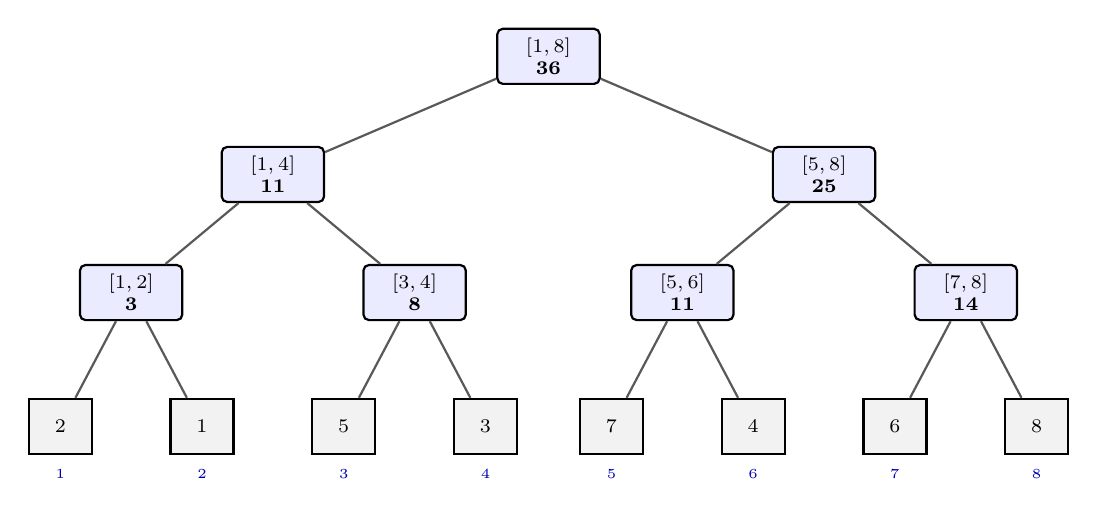
\begin{tikzpicture}[scale=1.0, every node/.style={transform shape}]
  \node[draw, thick, fill=blue!8, rounded corners=2pt, minimum width=1.3cm, minimum height=0.7cm, align=center, font=\scriptsize, inner sep=1pt] (n1) at (7, 6)   {$[1,8]$\\\textbf{36}};
  \node[draw, thick, fill=blue!8, rounded corners=2pt, minimum width=1.3cm, minimum height=0.7cm, align=center, font=\scriptsize, inner sep=1pt] (n2) at (3.5,4.5){$[1,4]$\\\textbf{11}};
  \node[draw, thick, fill=blue!8, rounded corners=2pt, minimum width=1.3cm, minimum height=0.7cm, align=center, font=\scriptsize, inner sep=1pt] (n3) at (10.5,4.5){$[5,8]$\\\textbf{25}};
  \node[draw, thick, fill=blue!8, rounded corners=2pt, minimum width=1.3cm, minimum height=0.7cm, align=center, font=\scriptsize, inner sep=1pt] (n4) at (1.7,3)  {$[1,2]$\\\textbf{3}};
  \node[draw, thick, fill=blue!8, rounded corners=2pt, minimum width=1.3cm, minimum height=0.7cm, align=center, font=\scriptsize, inner sep=1pt] (n5) at (5.3,3)  {$[3,4]$\\\textbf{8}};
  \node[draw, thick, fill=blue!8, rounded corners=2pt, minimum width=1.3cm, minimum height=0.7cm, align=center, font=\scriptsize, inner sep=1pt] (n6) at (8.7,3)  {$[5,6]$\\\textbf{11}};
  \node[draw, thick, fill=blue!8, rounded corners=2pt, minimum width=1.3cm, minimum height=0.7cm, align=center, font=\scriptsize, inner sep=1pt] (n7) at (12.3,3) {$[7,8]$\\\textbf{14}};
  \node[draw, thick, fill=gray!10, minimum width=0.8cm, minimum height=0.7cm, align=center, font=\scriptsize, inner sep=1pt] (l1) at (0.8,1.3) {2};
  \node[draw, thick, fill=gray!10, minimum width=0.8cm, minimum height=0.7cm, align=center, font=\scriptsize, inner sep=1pt] (l2) at (2.6,1.3) {1};
  \node[draw, thick, fill=gray!10, minimum width=0.8cm, minimum height=0.7cm, align=center, font=\scriptsize, inner sep=1pt] (l3) at (4.4,1.3) {5};
  \node[draw, thick, fill=gray!10, minimum width=0.8cm, minimum height=0.7cm, align=center, font=\scriptsize, inner sep=1pt] (l4) at (6.2,1.3) {3};
  \node[draw, thick, fill=gray!10, minimum width=0.8cm, minimum height=0.7cm, align=center, font=\scriptsize, inner sep=1pt] (l5) at (7.8,1.3) {7};
  \node[draw, thick, fill=gray!10, minimum width=0.8cm, minimum height=0.7cm, align=center, font=\scriptsize, inner sep=1pt] (l6) at (9.6,1.3) {4};
  \node[draw, thick, fill=gray!10, minimum width=0.8cm, minimum height=0.7cm, align=center, font=\scriptsize, inner sep=1pt] (l7) at (11.4,1.3){6};
  \node[draw, thick, fill=gray!10, minimum width=0.8cm, minimum height=0.7cm, align=center, font=\scriptsize, inner sep=1pt] (l8) at (13.2,1.3){8};
  \draw[draw, thick, color=gray!70!black] (n4)--(l1); \draw[draw, thick, color=gray!70!black] (n4)--(l2);
  \draw[draw, thick, color=gray!70!black] (n5)--(l3); \draw[draw, thick, color=gray!70!black] (n5)--(l4);
  \draw[draw, thick, color=gray!70!black] (n6)--(l5); \draw[draw, thick, color=gray!70!black] (n6)--(l6);
  \draw[draw, thick, color=gray!70!black] (n7)--(l7); \draw[draw, thick, color=gray!70!black] (n7)--(l8);
  \draw[draw, thick, color=gray!70!black] (n2)--(n4); \draw[draw, thick, color=gray!70!black] (n2)--(n5);
  \draw[draw, thick, color=gray!70!black] (n3)--(n6); \draw[draw, thick, color=gray!70!black] (n3)--(n7);
  \draw[draw, thick, color=gray!70!black] (n1)--(n2); \draw[draw, thick, color=gray!70!black] (n1)--(n3);
  \foreach \x/\i in {0.8/1, 2.6/2, 4.4/3, 6.2/4, 7.8/5, 9.6/6, 11.4/7, 13.2/8}
    \node[font=\tiny, text=blue!70!black] at (\x, 0.7) {\i};
\end{tikzpicture}
\caption{Segment Tree built over $A = [2,1,5,3,7,4,6,8]$. Each parent stores the sum of its two children.}
\label{fig:build}
\end{figure}

\subsection{Construction Complexity}
Since every node is visited and computed exactly once, the number of operations satisfies the recurrence

\begin{equation}
T(n) = 2T(n/2) + O(1),
\end{equation}

which, by the Master Theorem, gives

\begin{equation}
\boxed{T_{\text{build}}(n) = O(n)}.
\end{equation}

The tree itself occupies $O(n)$ space.

% ============================================================
\chapter{Point Update}

\subsection{Update Procedure}
An update replaces a single array value, $A[i] \leftarrow v$, and must restore correctness at every ancestor of leaf $i$. The procedure has two phases: a downward phase that locates the correct leaf, and an upward phase that recomputes each ancestor's summary.

\paragraph{Downward phase.} At a node representing $[lo, hi]$ with $mid = \lfloor (lo+hi)/2 \rfloor$, the target index $i$ falls into exactly one half:
\begin{itemize}[nosep]
  \item if $i \le mid$, recurse into the left child;
  \item otherwise, recurse into the right child.
\end{itemize}
This continues until a leaf $[i,i]$ is reached, whose value is set to $v$.

\paragraph{Upward phase.} As the recursion unwinds, every ancestor on the path recomputes its summary using Equation~\eqref{eq:merge}, combining its (possibly changed) two children.

\subsection{Example: update(4, 10)}
Starting from $A = [2,1,5,3,7,4,6,8]$, consider $\operatorname{update}(4,10)$, which changes $A[4]$ from $3$ to $10$, giving

\begin{equation}
A = [2,1,5,10,7,4,6,8].
\end{equation}

The downward path from the root follows

\begin{equation}
[1,8] \;\rightarrow\; [1,4] \;\rightarrow\; [3,4] \;\rightarrow\; \text{index } 4,
\end{equation}

since $4 \le mid = 4$ at the root, $4 \le mid = 2$ fails at $[1,4]$ (so we go right into $[3,4]$), and finally $4 \le mid = 3$ fails at $[3,4]$ (so we go right to the leaf).

On the way back up, each ancestor's summary is recomputed:

\begin{align}
S(3,4) &= 5 + 10 = 15, \\
S(1,4) &= S(1,2) + S(3,4) = 3 + 15 = 18, \\
S(1,8) &= S(1,4) + S(5,8) = 18 + 25 = 43.
\end{align}

The root's stored value therefore changes from $36$ to $43$, matching the net change of $+7$ introduced by replacing $3$ with $10$.

\subsection{Correctness of the Update}
Correctness follows directly from Equation~\eqref{eq:merge}: only nodes whose interval contains index $i$ can be affected by the change, and every such node lies on the unique root-to-leaf path to leaf $i$. Recomputing exactly this path, bottom-up, is therefore both necessary and sufficient to restore the invariant $S(l,r) = \sum_{i=l}^r A[i]$ at every node.

\subsection{Complexity Analysis}
Only a single root-to-leaf path is traversed, and the tree has height $h = \lceil \log_2 n \rceil$. Hence

\begin{equation}
\boxed{T_{\text{update}}(n) = O(\log n)}.
\end{equation}

% ============================================================
\chapter{Range Query}

\subsection{Three Cases}
To answer $Q(l,r)$, the query procedure compares the interval $[lo,hi]$ of the current node against the query range $[l,r]$ and falls into exactly one of three cases:

\begin{enumerate}[nosep]
  \item \textbf{Disjoint:} $[lo,hi] \cap [l,r] = \varnothing$. The node contributes nothing to the answer.
  \item \textbf{Completely contained:} $[l,r] \supseteq [lo,hi]$. The node's stored summary can be returned immediately, with no further traversal.
  \item \textbf{Partial overlap:} otherwise, both children must be explored recursively.
\end{enumerate}

\subsection{Query Procedure}
Formally, for a node $v$ representing $[lo,hi]$ with children $v_L, v_R$,

\begin{equation}
Q(v,l,r) =
\begin{cases}
0, & [lo,hi] \cap [l,r] = \varnothing, \\[4pt]
S(v), & [lo,hi] \subseteq [l,r], \\[4pt]
Q(v_L,l,r) + Q(v_R,l,r), & \text{otherwise.}
\end{cases}
\label{eq:query}
\end{equation}

\subsection{Example: sum(3, 7)}
On the updated array $A = [2,1,5,10,7,4,6,8]$, consider $Q(3,7)$. Applying Equation~\eqref{eq:query} from the root, the query range decomposes into three fully-contained segments:

\begin{equation}
[3,7] = [3,4] \cup [5,6] \cup [7,7].
\end{equation}

Their stored/derived values are

\begin{equation}
S(3,4) = 15, \qquad S(5,6) = 11, \qquad A[7] = 6,
\end{equation}

so that

\begin{equation}
Q(3,7) = 15 + 11 + 6 = 32.
\end{equation}

Table~\ref{tab:decomp} traces every node visited during this query, following the classification rule in Section~5.1.

\begin{table}[h]
\centering
\caption{Node-by-node decomposition of $Q(3,7)$ on $A=[2,1,5,10,7,4,6,8]$.}
\label{tab:decomp}
\begin{tabular}{lcr}
\toprule
\textbf{Visited segment} & \textbf{Status} & \textbf{Contribution} \\
\midrule
$[1,8]$ & Partial   & --- \\
$[1,4]$ & Partial   & --- \\
$[1,2]$ & Disjoint  & $0$ \\
$[3,4]$ & Contained & $15$ \\
$[5,8]$ & Partial   & --- \\
$[5,6]$ & Contained & $11$ \\
$[7,8]$ & Partial   & --- \\
$[7,7]$ & Contained & $6$ \\
\midrule
\textbf{Total} & & \textbf{32} \\
\bottomrule
\end{tabular}
\end{table}

As Table~\ref{tab:decomp} shows, $8$ of the tree's $15$ nodes were visited to answer this query; the remaining $7$ nodes (e.g.\ the leaves $1$ and $2$ beneath $[1,2]$, and leaf $8$ beneath $[7,8]$) are pruned without further recursion once their ancestor is classified as disjoint or fully contained.

\subsection{Complexity Analysis}
\label{sec:overlap-argument}
At any level of the Segment Tree, the query interval has at most two boundary regions that can partially overlap tree segments --- one near the left boundary and one near the right boundary. All other segments encountered at that level are either completely contained in the query interval or completely disjoint from it, and both of those cases terminate the recursion immediately by Equation~\eqref{eq:query}. Consequently, at most $O(1)$ partially-overlapping nodes are expanded per level, and since the tree has $O(\log n)$ levels,

\begin{equation}
\boxed{T_{\text{query}}(n) = O(\log n)}.
\end{equation}

% ============================================================
\chapter{Correctness and Design Reasoning}

\subsection{Invariant Maintained by Every Node}
The fundamental invariant is simple: every node stores the correct aggregate for exactly the interval represented by that node. For a sum tree, a node covering $[l,r]$ must contain $\sum_{i=l}^{r}A[i]$. This invariant is established during construction and preserved by every point update because only affected ancestors are recomputed from already-correct children.

\subsection{Why the Query Procedure Is Correct}
A range query partitions the requested interval into a collection of disjoint tree intervals. If a node is fully contained in the query range, its stored value is already exactly the contribution required. If it is disjoint, it contributes nothing. Partial overlap is resolved recursively until the relevant pieces become fully covered or disjoint. Because the selected nodes are disjoint and collectively cover the requested range, merging their summaries produces the exact answer.

\subsection{Why the Update Procedure Is Correct}
Suppose $A[i]$ changes. Only intervals containing index $i$ can have a different aggregate. The recursive update descends to the leaf representing $i$, writes the new value, and recomputes each ancestor from its two children. Every unaffected subtree retains its previous correct summary. Therefore, after returning to the root, the invariant holds throughout the tree again.

\begin{table}[H]
\centering
\caption{Correctness invariants for the principal operations.}
\label{tab:invariants}
\begin{tabular}{p{3.2cm}p{9.1cm}}
\toprule
\textbf{Operation} & \textbf{Invariant / postcondition}\\
\midrule
Build & Every node contains the aggregate of exactly its represented interval.\\
Point update & Every node on the root-to-updated-leaf path is recomputed; all other nodes remain valid.\\
Range query & Returned node summaries are disjoint and together cover exactly the requested interval.\\
Merge & Parent summary equals the merge of the summaries of its two child intervals.\\
\bottomrule
\end{tabular}
\end{table}

% ============================================================
\chapter{Implementation Design and Practical Issues}

\subsection{Array-Based Representation}
Although the conceptual model is a binary tree, a Segment Tree is commonly stored in a flat array. With one-indexed nodes, the left child of node $p$ is $2p$ and the right child is $2p+1$. This avoids explicit pointer objects and makes traversal inexpensive. A size of approximately $4n$ is a common safe allocation for a recursive implementation, although tighter layouts are possible.

\subsection{Indexing Conventions}
Implementations must consistently choose either zero-based or one-based indexing. Mixing conventions is a frequent source of off-by-one errors. In this report the mathematical exposition uses intervals such as $[1,n]$, while code may use the same convention for clarity. When adapting the algorithms to a programming language with zero-based arrays, the interval becomes $[0,n-1]$ and the midpoint and child ranges must be adjusted consistently.

\subsection{Recursive Versus Iterative Implementations}
A recursive implementation closely mirrors the mathematical definition and is often easier to verify. An iterative implementation can reduce function-call overhead and is useful when performance constraints or language limitations make recursion inconvenient. Both approaches rely on the same interval decomposition principle; the difference is primarily in how the traversal state is represented.

\subsection{Engineering Considerations}
For large values, the type used for node summaries matters. A sum may exceed the range of a 32-bit integer even when every individual element fits in that type, so 64-bit integers are commonly preferable. Memory allocation should also account for the chosen indexing scheme. In production code, input/output efficiency, cache behavior, recursion depth, and validation of query bounds can matter in addition to asymptotic complexity.

\begin{table}[H]
\centering
\caption{Common implementation concerns and their consequences.}
\label{tab:implementation}
\begin{tabular}{p{4cm}p{3.1cm}p{5.2cm}}
\toprule
\textbf{Concern} & \textbf{Typical choice} & \textbf{Reason}\\
\midrule
Node storage & Flat array & Low overhead and predictable memory access.\\
Tree allocation & About $4n$ & Simple safe bound for recursive layouts.\\
Numeric type & 64-bit integer & Reduces overflow risk for large aggregates.\\
Indexing & Consistent convention & Prevents boundary and midpoint errors.\\
Recursion & Depth $O(\log n)$ & Usually safe for normal Segment Tree heights.\\
\bottomrule
\end{tabular}
\end{table}

% ============================================================
\chapter{Advanced Extensions}

\subsection{Lazy Propagation}
When updates affect an entire interval rather than a single position, updating every affected leaf would defeat the purpose of the data structure. Lazy propagation addresses this by storing a deferred update at an internal node. The update is applied to the node's aggregate immediately, while a marker records that its children should receive the same change if they are visited later. With an appropriate node representation, range updates and range queries can both be supported in $O(\log n)$ time.

\subsection{Different Stored Summaries}
A node does not have to store one scalar. It may store a small structure containing several statistics, provided those statistics can be merged efficiently. For example, a node can maintain a total sum together with a maximum prefix sum, maximum suffix sum, and maximum subarray sum. This turns the Segment Tree into a framework for more sophisticated interval algorithms rather than merely a range-sum container.

\subsection{When a Segment Tree Is Not Necessary}
A Segment Tree is not automatically the right choice for every range problem. If there are no updates, prefix sums may answer range sums in $O(1)$ after preprocessing. If the operation is addition and only point updates and prefix/range sums are needed, a Fenwick Tree can provide the required asymptotic bounds with less memory. If the problem has special monotonic structure, specialized techniques may be simpler still. Data-structure selection should therefore follow the exact operation set rather than the popularity of a particular technique.

\subsection{Design Checklist}
Before implementing a Segment Tree, it is useful to identify the interval domain, the query operation, the update operation, the identity element if needed, and the exact information that must be stored at each node. This design step often determines whether a simple Segment Tree is sufficient or whether an augmented structure is required.

\begin{table}[H]
\centering
\caption{Design checklist for selecting and implementing a Segment Tree.}
\label{tab:checklist}
\begin{tabular}{p{4.2cm}p{8.1cm}}
\toprule
\textbf{Question} & \textbf{Design implication}\\
\midrule
What is queried? & Defines the node summary and merge operation.\\
What is updated? & Determines whether point updates are enough or lazy propagation is needed.\\
Is the merge associative? & Determines whether interval summaries can be combined consistently.\\
Is an identity required? & Needed when recursive queries return neutral values for disjoint segments.\\
How large can values become? & Determines the numeric type and overflow strategy.\\
How large is $n$? & Determines memory allocation and whether recursion is practical.\\
\bottomrule
\end{tabular}
\end{table}

% ============================================================
\chapter{Generalization of Segment Trees}
\label{sec:generalization}

One of the most powerful properties of the Segment Tree is that its \emph{shape} never changes when the underlying problem changes --- only what each node stores, and how two nodes are combined, needs to be redefined. The key requirement on the merge operation $f$ is \textbf{associativity}:

\begin{equation}
f(f(a,b),c) = f(a,f(b,c)).
\end{equation}

Addition satisfies this since $(a+b)+c = a+(b+c)$, and so do $\min$ and $\max$, since $\min(\min(a,b),c) = \min(a,\min(b,c))$ and likewise for $\max$. For a Segment Tree storing a single aggregate value, associativity of the merge is what makes the summary independent of how the interval was split; in implementations that must return a neutral value for a disjoint segment (Case~1 of Equation~\eqref{eq:query}), an appropriate \emph{identity element} $e$ satisfying $f(x,e) = x$ is also required --- for example $e = 0$ for sum, or $e = +\infty$ for minimum. Table~\ref{tab:generalization} lists several associative operations that can be substituted directly into the same tree structure.

\begin{table}[h]
\centering
\caption{Segment Tree generalized to different associative merge operations.}
\label{tab:generalization}
\begin{tabular}{lll}
\toprule
\textbf{Problem} & \textbf{Node stores} & \textbf{Merge rule} \\
\midrule
Range Sum     & Sum         & $a+b$ \\
Range Minimum & Minimum     & $\min(a,b)$ \\
Range Maximum & Maximum     & $\max(a,b)$ \\
Range GCD     & GCD         & $\gcd(a,b)$ \\
\rowcolor{blue!10}
Any associative rule & Any summary & swap in the rule \\
\bottomrule
\end{tabular}
\end{table}

\subsection{Range Sum, Minimum, Maximum, and GCD}
In each case, the build, update, and query algorithms of Sections~4--6 remain \emph{structurally identical}; only the merge step (Equation~\eqref{eq:merge}) is replaced. For range minimum, a node stores the smallest value in its interval and merges via $\min$; for range maximum, the largest value via $\max$; for range GCD, the greatest common divisor of the interval via $\gcd$.

\subsection{Associative Merge Operations}
Because associativity is the only requirement, the same $O(n)$ build and $O(\log n)$ update/query bounds carry over unchanged to every operation in Table~\ref{tab:generalization} --- and to any other associative operation not listed. Mastering one structure therefore unlocks a broad class of range-query problems.

% ============================================================
\chapter{Applications}

Table~\ref{tab:applications} summarizes representative domains where the Segment Tree's core pattern --- \emph{summarize a range, then change part of it, repeatedly and at scale} --- arises naturally.

\begin{table}[h]
\centering
\caption{Representative applications of the Segment Tree.}
\label{tab:applications}
\begin{tabular}{p{3.1cm}p{4.3cm}p{5.3cm}}
\toprule
\textbf{Application} & \textbf{Dynamic data} & \textbf{Possible query} \\
\midrule
Financial time series & Prices over time & Sum/min/max over a time interval \\
Leaderboards & Player scores & Range statistics over score intervals \\
Scheduling \& booking & Time-slot availability & Aggregate availability over an interval \\
Analytics dashboards & Continuously changing measurements & Range minimum/maximum/sum \\
\bottomrule
\end{tabular}
\end{table}

\subsection{Time-Series Data}
In a system tracking financial instrument prices, the Segment Tree supports instant range-sum, range-min, or range-max queries over any contiguous time window, even as thousands of price updates arrive per second.

\subsection{Leaderboards}
The basic sum Segment Tree described in this report does not, by itself, answer rank or $k$-th-largest queries. However, the same tree structure can be \emph{augmented} to store score frequencies at each node (rather than a running sum), which allows rank queries and $k$-th-order-statistic lookups to be answered in $O(\log n)$, with score updates handled just as fast.

\subsection{Scheduling and Booking}
Similarly, locating or reserving a free contiguous range of seats or time slots is not something the plain sum Segment Tree provides out of the box. It requires an \emph{augmented} Segment Tree in which each node stores additional information --- such as the count of free slots, and the longest prefix/suffix/interior run of free slots within its interval --- so that availability queries and reservations can still be resolved in $O(\log n)$.

\subsection{Other Dynamic Range Problems}
More generally, any system that must repeatedly answer ``what is true across this range?'' while ``something inside the range keeps changing'' is a candidate for a Segment Tree, regardless of the specific domain.

% ============================================================
\chapter{Segment Tree vs.\ Other Data Structures}

\subsection{Na\"ive Array}
A plain array supports $O(1)$ point updates but $O(n)$ range queries, since every query must be answered by scanning.

\subsection{Prefix Sum}
A prefix-sum array supports $O(1)$ range-sum queries but $O(n)$ point updates, since a single change invalidates every subsequent prefix.

\subsection{Fenwick Tree}
A Fenwick Tree (Binary Indexed Tree) supports both point update and range-sum query in $O(\log n)$, with a smaller memory footprint ($\sim n$) and a simpler implementation than a Segment Tree. A standard Fenwick Tree is particularly well suited to prefix/range aggregation under operations such as addition, while Segment Trees provide a more general framework for associative range aggregates and accommodate range updates via lazy propagation considerably more naturally.

\subsection{Comparison Table}
Table~\ref{tab:comparison} summarizes the comparison. Rather than declaring one structure to be strictly superior, the appropriate conclusion is that Fenwick Trees generally use less memory and have a simpler implementation, while Segment Trees support a broader class of associative range operations and naturally accommodate extensions such as lazy propagation.

\begin{table}[h]
\centering
\caption{Segment Tree versus Fenwick Tree.}
\label{tab:comparison}
\begin{tabular}{lcc}
\toprule
\textbf{Property} & \textbf{Segment Tree} & \textbf{Fenwick Tree} \\
\midrule
Point update            & $O(\log n)$ & $O(\log n)$ \\
Range query              & $O(\log n)$ & $O(\log n)$ \\
Build                    & $O(n)$      & $O(n)$ \\
Typical memory           & $\sim 4n$   & $\sim n$ \\
Range minimum/maximum    & Flexible    & More restricted \\
Lazy range update        & Natural     & Not the basic operation \\
Implementation           & More complex& Simpler \\
\bottomrule
\end{tabular}
\end{table}

% ============================================================
\chapter{Complexity and Practical Considerations}

Table~\ref{tab:summary} consolidates the complexity results derived in Sections~4--6.

\begin{table}[h]
\centering
\caption{Summary of Segment Tree time and space complexity.}
\label{tab:summary}
\begin{tabular}{llp{6.5cm}}
\toprule
\textbf{Operation} & \textbf{Time Complexity} & \textbf{Explanation} \\
\midrule
Build         & $O(n)$      & Every tree node is constructed exactly once. \\
Point update  & $O(\log n)$ & Exactly one root-to-leaf path is recomputed. \\
Range query   & $O(\log n)$ & At most $O(1)$ partially-overlapping nodes are expanded per level (Section~\ref{sec:overlap-argument}). \\
Space         & $O(n)$      & The tree has a linear number of nodes. \\
\bottomrule
\end{tabular}
\end{table}

\begin{equation}
\boxed{
\begin{aligned}
\text{Build} &= O(n) \\
\text{Query} &= O(\log n) \\
\text{Update} &= O(\log n) \\
\text{Space} &= O(n)
\end{aligned}}
\end{equation}

As a purely illustrative, hypothetical operation-count comparison (not a benchmark of any real implementation): assuming a system with $n = 1024$ instruments processes $q = 36 \times 10^9$ combined queries and updates, and that each elementary step takes roughly $1$ nanosecond, an $O(qn)$ na\"ive approach would require on the order of $10.24$ hours of raw operation count, whereas an $O(q \log n)$ Segment Tree approach would require on the order of $6$ minutes. The gap is driven entirely by $n$ versus $\log_2 n$ in the operation count, and the absolute times should be read only as an order-of-magnitude illustration rather than a measured runtime.

% ============================================================
\chapter{Conclusion}

The Segment Tree resolves the fundamental tension between fast range queries and fast point updates by recursively decomposing an array into a hierarchy of intervals, each summarized at a tree node. This organization allows both operations to be performed in $O(\log n)$ time after an $O(n)$ build, as proven via the overlap argument for queries and the single-path argument for updates. Because the only requirement on the merge operation is associativity, the same structure generalizes immediately to range minimum, maximum, GCD, and a wide class of other problems, which is what makes the Segment Tree applicable across domains as different as financial time series, live leaderboards, and scheduling systems. Compared to a Fenwick Tree, a Segment Tree trades some memory and implementation simplicity for substantially greater flexibility, making the choice between the two ultimately dependent on what a given problem demands.

% ============================================================
\appendix
\chapter{Reference Pseudocode}

The following compact templates summarize the three core routines described throughout the report. They intentionally expose the merge operation so that the same structure can be adapted to sums, minima, maxima, GCD, or another associative aggregate.

\begin{lstlisting}
build(node, lo, hi):
    if lo == hi:
        tree[node] = A[lo]
        return
    mid = (lo + hi) // 2
    build(2*node, lo, mid)
    build(2*node+1, mid+1, hi)
    tree[node] = merge(tree[2*node], tree[2*node+1])

update(node, lo, hi, pos, value):
    if lo == hi:
        tree[node] = value
        return
    mid = (lo + hi) // 2
    if pos <= mid:
        update(2*node, lo, mid, pos, value)
    else:
        update(2*node+1, mid+1, hi, pos, value)
    tree[node] = merge(tree[2*node], tree[2*node+1])

query(node, lo, hi, ql, qr):
    if qr < lo or hi < ql:
        return identity
    if ql <= lo and hi <= qr:
        return tree[node]
    mid = (lo + hi) // 2
    left = query(2*node, lo, mid, ql, qr)
    right = query(2*node+1, mid+1, hi, ql, qr)
    return merge(left, right)
\end{lstlisting}

\chapter{Summary of Complexity}
\begin{table}[H]
\centering
\caption{Final complexity reference.}
\begin{tabular}{lcc}
\toprule
\textbf{Operation} & \textbf{Time} & \textbf{Extra Space}\\
\midrule
Build & $O(n)$ & $O(n)$ tree storage\\
Point update & $O(\log n)$ & $O(\log n)$ recursion stack\\
Range query & $O(\log n)$ & $O(\log n)$ recursion stack\\
\bottomrule
\end{tabular}
\end{table}

\begin{thebibliography}{9}

\bibitem{clrs}
T.~H. Cormen, C.~E. Leiserson, R.~L. Rivest, and C.~Stein, \textit{Introduction to Algorithms}, MIT Press.

\bibitem{cphandbook}
A.~Laaksonen, \textit{Competitive Programmer's Handbook}.

\bibitem{cpalgorithms}
cp-algorithms, ``Segment Tree,'' \textit{Algorithms for Competitive Programming}. \url{https://cp-algorithms.com/data_structures/segment_tree.html}

\end{thebibliography}

\end{document}
